%
% Perspective
%

% !TEX root = ../../main.tex

\chapter{Diskussion und Ausblick\label{chap:perspective}}

  \todo[inline]{Bespricht die erzielten Ergebnisse bezüglich ihrer Erwartbarkeit, Aussagekraft und Relevanz}
  \todo[inline]{Interpretation und Validierung der Resultate}
  \todo[inline]{Rückblick auf Aufgabenstellung, erreicht bzw\@. nicht erreicht}
  \todo[inline]{Legt dar, wie an die Resultate (konkret vom Industriepartner oder weiteren
  Forschungsarbeiten; allgemein) angeschlossen werden kann; legt dar, welche Chancen die
  Resultate bieten}

  \section{Diskussion der Resultate\label{sec:diskRes}}

    Die gefundenen Resultate wiederspiegeln Lösungen innerhalb einer künstlichen Umgebung.
    In dieser Umgebung wird eine vereinfachte Physik verwendet, welche nur an die reale Physik angenähert ist.
    Deshalb sind die Resultate nicht ohne Vorbehalte auf die reale Welt übertragbar.
    \\
    Das Evolvieren von artifiziellen Tieren und ihrer Steuerung ist möglich mit dem implementierten evolutionären Algorithmus.
    Es entwickelte sich keine klassische Laufbewegung,
    aber eine Bewegung welche es den Individuen erlaubt sich durch den Parcours fortzubewegen.
    \\
    Es stellt sich heraus, dass eine Simulation viel Zeit beansprucht und äusserst rechenintensiv ist.
    12000 Generationen zu simulieren, dauert rund 10 Tage. \\
    Es kann die Hypothese aufgestellt werden, dass die JavaScript-Engine V8 momentan noch nicht ausreichend schnell ist.
    Eine weiterführende Arbeit kann untersuchen wie die Leistungen anderer Implementationen von Javascript-Engines im
    Vergleich zu V8 abschneiden.

    \subsection{Wie kann eine Steuerung der Bewegung implementiert werden?}

      % TODO Flo input
      Der~\vref{sec:Engine} beschreibt wie die Steuerung der Bewegung implementiert wurde.

    \subsection{Wie kann diese Steuerung evolviert werden?}

      % TODO Flo input
      Die Steuerung wurde durch Selektion und Mutation evolviert.

    \subsection{Wie kann die Geometrie der Tiere evolviert werden?}
      Die Konstruktion der geometrischen Körper aus deren sich ein Individuum zusammensetzt,
      wurde unter \vref{sub:Beine} und \vref{subsub:GenotypeBodypointCreation} besprochen.
      Welche Geometrie die richtige ist, wird durch die Selektion und Mutation der Individuen bestimmt.


    \subsection{Nimmt die Diversität mit zunehmenden Generationen stetig ab?}
      Analysiert man die Diversitätsgraphe aus dem vierten~(\vref{sec:4lauf}) und
      fünften Simmulationslauf~(\vref{sec:5lauf}) sieht man einen Abfall der Diversität in den ersten Generationen.
      Bei der allgemeinen Lösung erholt sich die Diversität mit zunehmenden Generationen.
      Gewisse Ausreisser erreichen sogar die Diversität der ersten Generationen.
      Jedoch zeichnet sich ein anderes Bild bei dem Evolvieren auf Evolvierbarkeit ab.
      Hier fällt die Fitness ab der 2000. Generation auf ein niedriges Niveau.
      Es hat sich gezeigt, dass die allgemeine Lösung diverse Individuen liefert.


    \subsection{Wie sieht der Bewegungsablauf und Geometrie eines evolvierten Tieres aus?}
      Neben der vordefinierten Bewegungsablauf~(\vref{sec:Engine}) wurden drei weitere Typen gefunden:
      \begin{itemize}
        \item Rollbewegung
        \item Hüpfbewegung
        \item Ruderbewegung
      \end{itemize}
      Bei der Rollbewegung drehen sich die Individuen einmal um sich selber. Die Gemoetrie des Körpers tendiert zu einer kreisartigen Form.
      %figure Rollen
      Die Hüpfbewegung führen die Individuen dadurch aus, dass sie sich mit einem Bein vom Boden abstossen.
      %%figur Hüpfbewegung
    \subsection{Individuum: Allgemeine Lösung vs Evolvieren auf Evolvierbarkeit}
      Es wird das beste Indivdiuum der 4000. Generation~(\vref{fig:gen4000}) aus dem vierten Simulationslauf~\vref{sec:4lauf}
      und dem füften Simulationslauf~(\vref{sec:5lauf}) miteinander verglichen.
      Die Individuen haben beide eine Hüpfbewegung entwickelt.
      Jedoch streckt das eine Individum~(\vref{fig:gen4000_alg}) alle Beine,
      während das Andere~(\vref{fig:gen4000_ev}) fast alle Beine angewinkelt hat.
      Ebenso weisst der Körper des Individuums, welches auf Evolvierbarkeit evolviert wurde, eine grössere Masse auf.
      Die Masse aller Beine ist folglich grösser beim Individum der allgemeinen Lösung.
      Die Steuerung beider Individuen sind also quasi identisch, während bei der Geometrie leichte Unterschiede festgestellt worden sind.

      \begin{figure}[H]
        \centering
        \begin{subfigure}[b]{0.45\textwidth}
          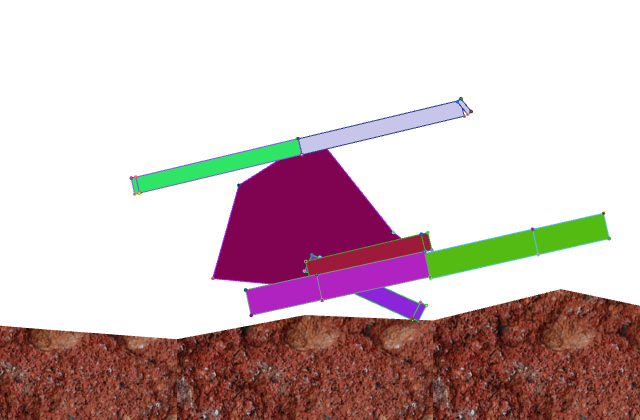
\includegraphics[width=\linewidth,center]{graphics/simulation-discussion/4_gen4000}
          \caption{Allgemeine Lösung\label{fig:gen4000_alg}}
        \end{subfigure}
        \begin{subfigure}[b]{0.45\textwidth}
          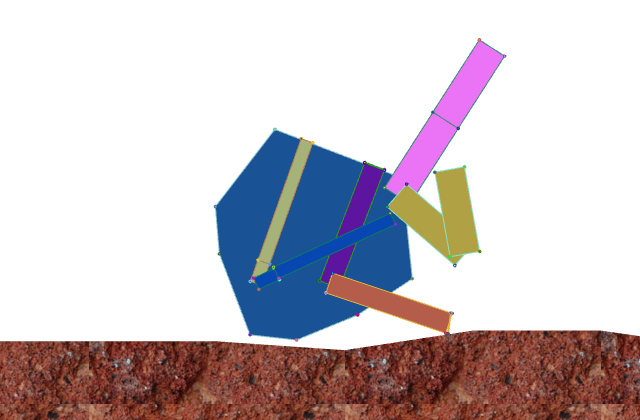
\includegraphics[width=\linewidth,center]{graphics/simulation-discussion/5_gen4000}
          \caption{Evolvierung auf Evolvierbarkeit\label{fig:gen4000_ev}}
        \end{subfigure}

        \caption{4000. Generation\label{fig:gen4000}}
      \end{figure}



    \subsection{Hypothese Körperpunkte}

      Um eine Aussage über die Hypothese der Körperpunkte~(\vref{subsub:hypoKp}) zu treffen,
      müsste wie erwähnt unter~\vref{subsub:bpScnd} die Mutation der Anzahl Körperpunkte implementiert werden.
      Spätestens ab der 10. Generation bei jedem Lauf,
      existieren nur noch Individuen mit der gleichen Anzahl Körperpunkten.

    \subsection{Hypothese Mutationswahrscheinlichkeiten}

      Die Hypothese über die Mutationswahrscheinlichkeiten~(\vref{subsub:hypoMut}) hat sich bewahrheitet
      wie in~\vref{subsub:3000gen} festgestellt worden ist.
      Mit kleineren Mutationswahrscheinlichkeiten lassen sich fittere Indivduen finden.

  \section{Ausblick\label{sec:ausblick}}

    % Tiere mit andere anzahl an beinen als 6

    Die erstelle Simulationsapplikation ist gut erweiterbar und ermöglicht Interessierten sie weiter auszubauen.
    Der Programmcode soll für Interessierte unter \url{http://github.com} freigegeben werden nach der Abgabe der Arbeit.

    \subsection{Feedback an den Bewegungsmotor\label{sec:PerspectiveFeedback}}

      Die fehlende Implementation der Reaktion auf das Feedback der Steuerung ist sicher die Komponente,
      welche am meisten helfen würde, bessere Resultate zu finden.

    \subsection{Austauschen der Physik-Engine}

      Eine Verbesserungsmöglichkeit ist die langsame und teilweise fehlerhafte \gls{PhysicsEngine} p2.js auszutauschen.
      Mit Hilfe einer anderen \gls{PhysicsEngine} kann schneller simuliert werden und es können bessere Resultate gefunden werden.
      Für einen 30 Sekunden langen Simulationslauf, benötigt die Engine zum Teil mehr als eine Minute.

    \subsection{Hypothese Selektionsstrategie\label{sub:hypoSelect}}

      Die zeitliche Beschränkung dieser Arbeit hat es nicht erlaubt,
      die ursprünglich geplante Hypothese über den Vergleich von Selektionsstrategien durchzuführen.
      In der Hypothese ging es darum die Auswirkungen von den Selektionsstrategien:
      Turnierbasierte-Selektion, rangbasierte Selektion
      und proportionale Selektion auf die Simulationsresultate zu untersuchen.
      Diese Hypothese würde genügend Stoff für eine weitere spannende Arbeit liefern.

    \subsection{Hypothese Allgemeine Lösung vs.\ Evolvierung auf Evolvierbarkeit\label{sub:hypoAnsatz}}

      Leider war nicht genügend Zeit vorhanden folgende Hypothese zu validieren:
      Individuen welche durch die allgemeine Lösung gefunden werden,
      sollten bei unterschiedlichen Parcours im Durchschnitt besser abschneiden,
      als ihre Gegenspieler~(Evolvierung auf Evolvierbarkeit),
      da sie sich schneller an eine neue Umgebung anpassen können.
      Wenn immer der gleiche Parcours benutzt wird,
      sollten die Individuen welche auf Evolvierbarkeit evolviert worden sind, auf Dauer überlegen sein.
      \\
      Um diese Hypothese zu validieren,
      sollten zwei Simulationsläufe mit zwei Populationen aus den Lösungsansätzen durchgeführt werden:

      \begin{itemize}
        \item Simulationslauf mit gleichem Parcours
        \item Simulationslauf mit 10 unterschiedlichen Parcours
      \end{itemize}

      Anschliessend sollte ein Vergleich angestellt werden zwischen den Lösungsansätzen der beiden Läufen.

    \subsection{Parcours}

      Der Parcours wird nur mit einem Typ von Element generiert, ein Höhenfeld welches einen Berg repräsentiert.
      Neue Terrain-Typen wie Eis, Wasser oder Grass könnten zusätzlich hinzugefügt werden.

      % Tendenz?
